\scanpage{64}
On trouve qu'ils correspondent au cas de \deleted{\unsure{un syst.}} la figure ci-contre, correspondant à un syst. transitif d'isom entre les $I_\alpha$ (définis par les triangles intersection $Y\cap X_\alpha$).

\diagram{\begin{tikzcd}[ampersand replacement=\&,column sep=tiny,row sep=tiny]
\&\& {}\arrow[dd,dash]\arrow[dl,dash]\\
{}\arrow[urr,dash]\arrow[r,dash]\arrow[dd,dash]\&{}\arrow[dd,dash]\&\\
\&\&{}\arrow[dd,dash]\arrow[dl,dash]\\
{}\arrow[urr,dash]\arrow[r,dash]\arrow[dd,dash]\&{}\arrow[dd,dash]\&\\
\&\&{}\arrow[dl,dash]\\
{}\arrow[urr,dash]\arrow[r,dash]\&{}\&
\end{tikzcd}}

Pour tt triangle donné de $X_\alpha$ (correspondant à une bijection $I_\beta\mathbin{\unsure{-|\longrightarrow}}I_\gamma$) il y en a 6.

\begin{center}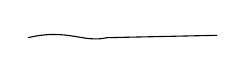
\begin{tikzpicture}\draw (0,0) .. controls (.5,.12) and (.7,-.07) .. (1,0) -- (2.4,.03);\end{tikzpicture}\end{center}

Étudier plus génér\textsuperscript{t}.

a) Position relative de 2 $\unsure{\mathscr T|\Gamma|\mathcal T}_i$ $(-1\le i\le1)$ dans un $\mathscr T_2$

b) Position relative d'une base et d'un $\mathscr T_i$.

\textcircled{20} (\unsure{Variante}) Soit $\tau=\{a,b,c\}$ une triade du $\mathscr T_2$ $\Delta=(S,A)$. Alors \deleted{\unsure{$B$ l'ens}} il y a exactement un bitriangle contenant $t$, qui est aussi formé des él. de $\tau$ et de \inserted{l'ens} des 6 él. de $S-\tau$ qui sont liés à \deleted{au moins} \inserted{exactement} \deleted{\unsure{un}} \inserted{deux} él. de $\tau$ \deleted{(ils sont liés \unsure{en|aux} \inserted{alors}, en fait, à deux tels éléments)}.
Alors $X-\tau=Y$ est un \deleted{hexagone} \unsure{bitripode|bitriade|distingué} i.e. un hexagone. On trouve ainsi une bijection de l'ens des triades sur l'ens des hexagones.

% archive sheet number: 63

